\documentclass[10pt,letterpaper]{article}
\usepackage[T1]{fontenc}
\usepackage{times,microtype,graphicx,booktabs,float}
\usepackage[font=small,labelfont=bf,labelsep=period,skip=4pt]{caption}
\setlength{\textwidth}{6in}
\setlength{\textheight}{9in}
\setlength{\oddsidemargin}{0.25in}
\setlength{\evensidemargin}{0.25in}
\setlength{\topmargin}{-0.35in}
\setlength{\headheight}{0.15in}
\setlength{\headsep}{0.2in}
\setlength{\parindent}{0pt}
\setlength{\parskip}{4pt}
\setlength{\intextsep}{4pt}
\setlength{\textfloatsep}{9pt}
\newcommand{\reporttitle}[2]{\noindent\rule{\linewidth}{4pt}\par
{\LARGE\bfseries #1\par}\vspace{2pt}\noindent\rule{\linewidth}{1pt}\par
#2\par October 16, 2026\par\vspace{4pt}}
\makeatletter
\renewcommand\section{\@startsection{section}{1}{\z@}{9pt}{4pt}{\large\bfseries}}
\makeatother
\renewenvironment{abstract}{\small\textbf{Abstract}\par}{\par\vspace{3pt}}
\let\originalitemize\itemize
\renewcommand{\itemize}{\originalitemize\setlength{\itemsep}{1pt}\setlength{\parskip}{0pt}\setlength{\parsep}{0pt}}
\let\originalenumerate\enumerate
\renewcommand{\enumerate}{\originalenumerate\setlength{\itemsep}{1pt}\setlength{\parskip}{0pt}\setlength{\parsep}{0pt}}
\begin{document}
\reporttitle{Peak calling package comparison}{Arabidopsis DAP and ATAC; caller policies and optimized MACS3}
\begin{abstract}MACS2 and MACS3 give similar independent motif support in two SE DAP treatments, while Genrich produces zero peaks at the tested q = 0.01 operating point. A separate optimized-MACS3 test preserves outputs in all 24 comparisons and reduces wall time by 4.20 to 42.79 times across CPU settings. Genrich thresholds are not statistically interchangeable with MACS thresholds, and parallel MACS3 uses more sampled memory. We would retain caller policies and support the pinned optimization within the tested scope.\end{abstract}
\section*{Setup}
\textbf{Data.} The method matrix uses 1-million and 5-million raw-template caps. The separate optimization uses 8 existing treatment/replicate input cases across SE DAP, PE DAP and ATAC, with fixed controls and input hashes.

\textbf{Scoring.} Peak discovery is reported with union coverage and biological replicate overlap, not treated as accuracy. Held-out FRiP uses the other replicate's peaks. Exact optimized-output equivalence compares narrowPeak/summit bytes and peak-table content excluding header comments.

\begin{table}[H]\centering\small\caption{Input identities at the dap-se-5m cap.}
\begin{tabular}{lrr}\toprule
Library & Role / control & Raw templates \\ \midrule
SRR2926068 & Control & 4,241,389 \\
SRR2926076 & SRR2926068 & 5,000,000 \\
SRR2926841 & SRR2926068 & 5,000,000 \\
\bottomrule\end{tabular}\end{table}
\section{Greater depth improves measured ATAC replicate agreement}
Across 2 biological replicates, TAIR10 peak-base Jaccard rises from 0.2404 to 0.4858 between 1 million and 5 million pairs. Peak discovery rises from 4,997 to 14,805 and from 3,043 to 11,551, so greater held-out FRiP is interpreted alongside expanded peak coverage.

\begin{figure}[H]\centering\makebox[\linewidth][c]{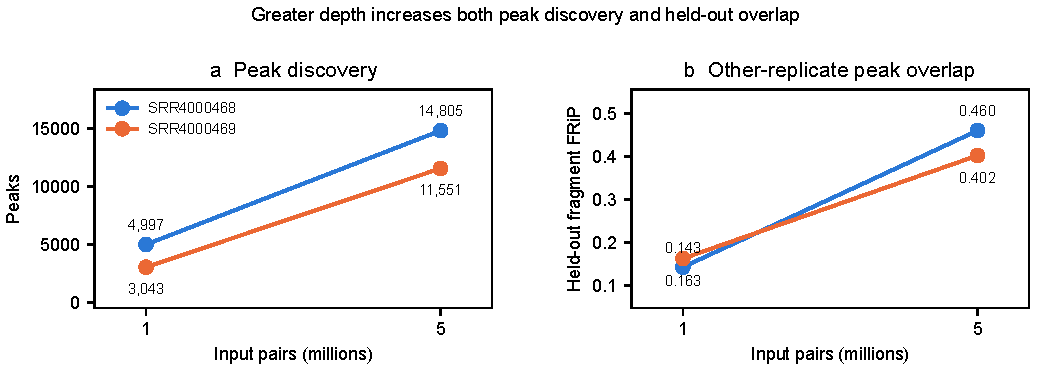
\includegraphics[width=7in]{figures/depth.pdf}}
\caption{Depth-dependent peak discovery and held-out fragment overlap.}\end{figure}
\newpage
\section{Caller operating points prevent a simple accuracy ranking}
At q = 0.01, Genrich reports 0 peaks for both ATAC replicates at both tested depths. Diagnostic p = 0.01 calls are a different operating point, not a rescue at a matched false-discovery rate.

\begin{table}[H]\centering\small\caption{Recorded median measurements; nd means not determined.}
\begin{tabular}{lrrrr}\toprule
Method & Library & Peaks & Union bp & Own FRiP \\ \midrule
baseline & SRR4000468 & 4,997 & 1,981,744 & 0.2587 \\
baseline & SRR4000469 & 3,043 & 1,550,760 & 0.1466 \\
macs2 & SRR4000468 & 4,997 & 1,981,744 & 0.2587 \\
macs2 & SRR4000469 & 3,043 & 1,550,760 & 0.1466 \\
genrich & SRR4000468 & 0 & 0 & 0.0000 \\
genrich & SRR4000469 & 0 & 0 & 0.0000 \\
\bottomrule\end{tabular}\end{table}
\begin{table}[H]\centering\small\caption{Independent motif support at the deeper SE DAP cap.}
\begin{tabular}{lrr}\toprule
Library & Caller & PBM hits / matched windows \\ \midrule
SRR2926076 & macs2 & 468/998 \\
SRR2926076 & baseline & 466/998 \\
SRR2926841 & macs2 & 582/1000 \\
SRR2926841 & baseline & 581/1000 \\
\bottomrule\end{tabular}\end{table}
\textbf{Policies.} MACS2 2.2.9.1 and MACS3 3.0.5 use BAM for SE and BAMPE for PE, with assigned DAP controls and keep-dup = 1; ATAC retains all already-filtered fragments. Genrich 0.6.2 uses ATAC cut-site mode, 100-base expansion, AUC 200 and gap 100. Its background includes header contigs, whereas the ATAC MACS effective size uses nuclear ACGT bases.

\textbf{Reproducibility.} Exploratory pairwise IDR uses permissive MACS p = 0.01 calls, signal-value ranking and seed 60141. There are no pooled/pseudoreplicate rescue ratios or approved plant exclusion thresholds; this is not an ENCODE acceptance claim.

\section{The optimization preserves the evaluated peak outputs}
All 24 CPU-specific comparisons pass output equivalence across 8 inputs. The 192 invocations comprise 48 warmups and 144 measured calls, with 3 measured repetitions per build and CPU setting.

\begin{table}[H]\centering\small\caption{Paired optimized/released comparisons on identical input files.}
\begin{tabular}{lrr}\toprule
Allocated CPUs & Wall-time speedup range & RSS direction \\ \midrule
1 & 4.20 to 6.32 & Lower in all 8 \\
2 & 7.98 to 16.94 & Case-dependent \\
8 & 9.07 to 42.79 & Higher in all 8 \\
\bottomrule\end{tabular}\end{table}
\newpage
\section{Parallel speed gains require additional sampled memory}
For the largest tested PE DAP case at 8 CPUs, median wall time falls from 84.29 to 1.97 seconds while sampled group RSS rises from 639 to 1,330 MiB. At 1 CPU, all 8 inputs instead show lower sampled RSS with the optimized build.

\begin{figure}[H]\centering\makebox[\linewidth][c]{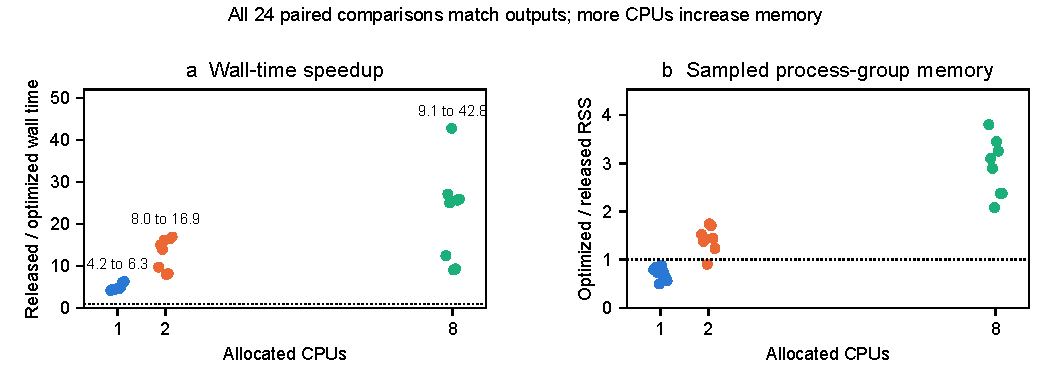
\includegraphics[width=7in]{figures/macs-speed.pdf}}
\caption{Paired speed and sampled-memory ratios across eight input cases.}\end{figure}
\textbf{Build identity.} The released and optimized binaries both report 3.0.5. The optimized source is pinned to 22eb40f7b51f5b20b635614ca0b1759dc5398c5c, with matched Python and numerical dependencies; the release number alone cannot identify this optimization. Measurements use a nonexclusive x86-64 Xeon host, CPU affinity, one warmup and three measured runs.

\section*{Open issues}
\begin{itemize}
\item Sampled process-group RSS can double-count shared pages and is not host peak RAM.
\item The PE DAP 5M treatment cap contains 1,657,793 actual pairs; its control contains 5M.
\item The SE DAP 5M control contains 4,241,389 reads, not 5M.
\item The upstream suite has one call-variant failure also seen in the release; it is not fully green.
\end{itemize}
\section*{Recommendation}
We would support the pinned optimized caller as a scoped opt-in and retain scientific peak-calling policies.

\begin{enumerate}
\item Validate the published deployment image and representative full-depth inputs before promotion.
\item Compare callers using independent support and biological reproducibility at declared operating points.
\end{enumerate}
\section*{Appendix: Methods}
We summarize recorded results without rerunning biological processing. The main Arabidopsis matrix uses seeded nested raw-template subsets (seed 60141), three fresh technical repetitions at the 1-million cap and one at the 5-million cap. Actual counts replace requested caps for short libraries. DAP retains primary mapped reads including MAPQ 0; ATAC selects proper primary pairs with both mates MAPQ at least 30, excludes MAPQ 255, organelles and marked duplicates. Biological identity is preserved. Source files are SHA-256 checked against the accompanying catalog; evidence snapshot revision ed1c50b8e4b5 includes the October 13 to 16 records. Completed local reference assessments are separately identified in that catalog.

\end{document}
